问题一从两束反射光的相位差出发。若波数为 $\nu$，外延层厚度为 $d$，折射率为 $n$，折射角为 $\theta_t$，则相位项可写成
\[
\phi(\nu)=4\pi n d \cos(\theta_t)\nu+\phi_0 .
\]
因此反射率曲线在波数域的主频满足
\[
f=2nd\cos(\theta_t).
\]
由 Snell 定律有 $\theta_t=\arcsin(\sin\theta/n)$，于是厚度可由
\[
d=\frac{f}{2n\cos(\theta_t)}
\]
得到。若 $d$ 先以 cm 表示，则乘以 $10^4$ 转换为 um。图 \ref{fig:q1schematic} 给出这一反演链条。该模型的朴素基线是直接使用相邻峰间距 $\Delta\nu$，即 $d=1/(2n\cos\theta_t\Delta\nu)$。主模型则通过整段光谱拟合主频，减少单个峰检测误差的影响。

这个公式也解释了为什么同一厚度在不同入射角下可以相互校验。入射角改变后，折射角 $\theta_t$ 和 $\cos(\theta_t)$ 会改变，光谱条纹周期也会随之改变；但只要折射率和厚度模型正确，经过角度修正后反演出的 $d$ 应该回到同一数值附近。若两组角度差异明显，通常意味着三类问题之一：一是峰值间距识别错误，二是单位换算或角度换算错误，三是单光束模型已经不足以解释数据。这个判断逻辑比单独报告一个厚度值更适合作为回归测试。

在本案例中，峰间距法不是最终答案，而是基线。它的优势是透明，能用相邻峰差直接估计厚度量级；缺点是对局部峰值位置敏感。最小二乘频率拟合则把整条曲线的振荡信息一起使用，能降低单点峰值误差带来的波动。两者搭配后，可以同时满足可解释性和数值稳定性要求。

\begin{figure}[htbp]
\centering

\includegraphics[width=0.86\textwidth]{../figures/fig_q1_model_schematic.png}
\caption{问题一的单光束干涉厚度反演模型示意。}
\label{fig:q1schematic}
\end{figure}

\begin{figure}[htbp]
\centering
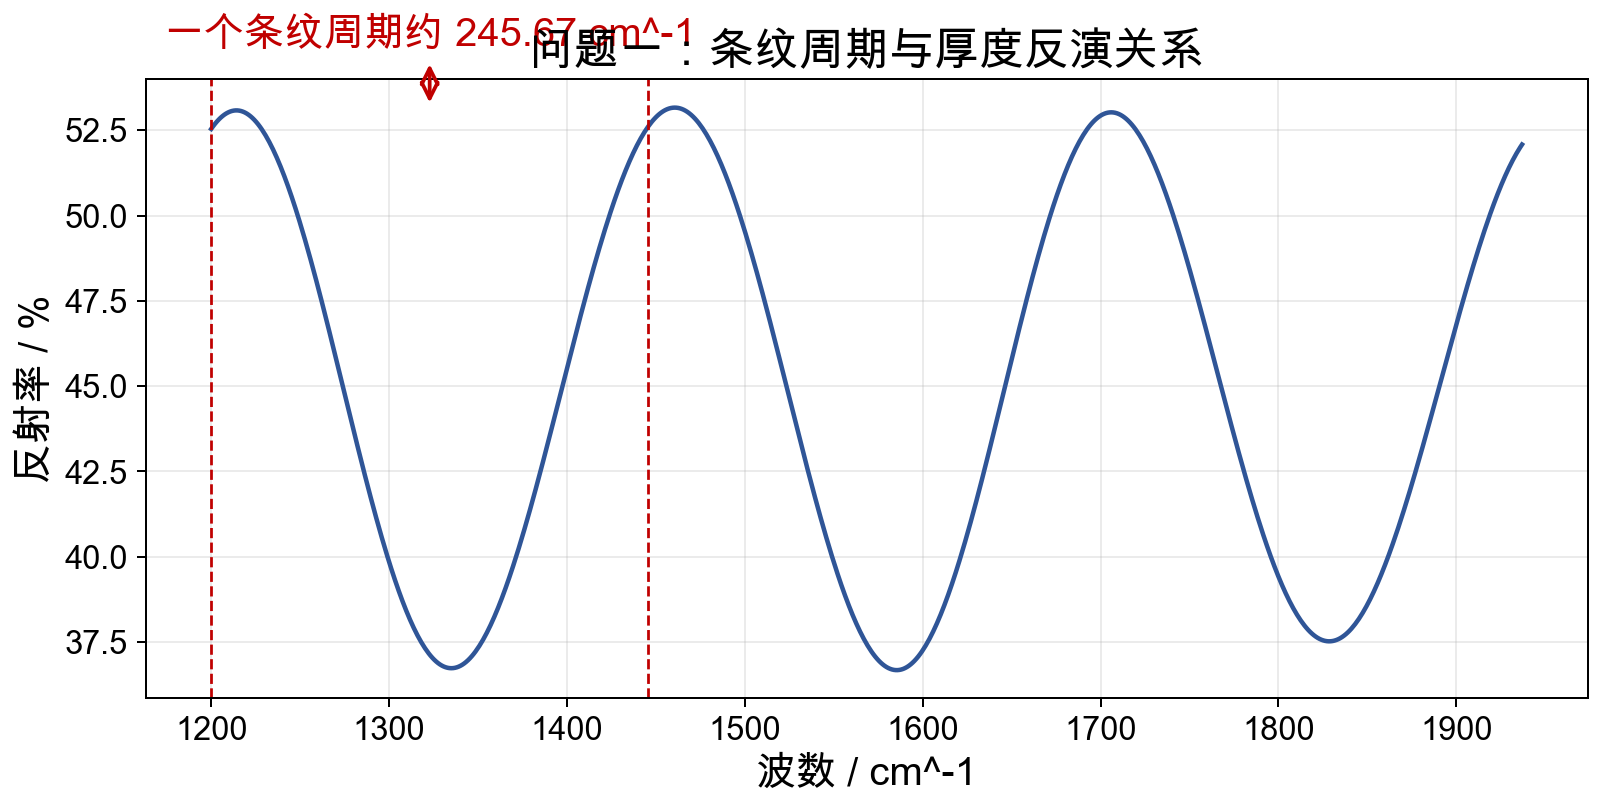
\includegraphics[width=0.86\textwidth]{../figures/fig_q1_result.png}
\caption{问题一中条纹周期和厚度反演关系的合成光谱示例。}
\label{fig:q1result}
\end{figure}
